% Created 2018-01-13 Sat 08:35
\documentclass{foils}
\usepackage[utf8]{inputenc}
\usepackage[T1]{fontenc}
\usepackage{fixltx2e}
\usepackage{graphicx}
\usepackage{longtable}
\usepackage{float}
\usepackage{wrapfig}
\usepackage{rotating}
\usepackage[normalem]{ulem}
\usepackage{amsmath}
\usepackage{textcomp}
\usepackage{marvosym}
\usepackage{wasysym}
\usepackage{amssymb}
\usepackage{hyperref}
\tolerance=1000
\author{Thomas J. Faulkenberry, Ph.D.}
\date{Jan 16, 2018}
\title{PSYC 5301 - Week 1}
\hypersetup{
  pdfkeywords={},
  pdfsubject={},
  pdfcreator={Emacs 25.3.1 (Org mode 8.2.10)}}
\begin{document}

\maketitle

\foilhead{An example}
\label{sec-1}
Suppose you have a treatment that you suspect may alter performance on a certain task.  The two groups were significantly different, $t(18)=2.7$, $p=0.01$.  Decide whether each of the following statements is true or false:
\begin{enumerate}
\item You have disproved the null hypothesis
\item You have found the probability of the null hypothesis being true
\item You have proved your experimental hypothesis
\item You can deduce the probability of the experimental hypothesis being true
\item If you decide to reject the null hypothesis, you know the probability that you are making the wrong decision
\item You have a reliable experimental finding in the sense that if, hypothetically, the experiment were repeated a large number of times, you would obtain a significant result on 99\% of the replications.
\end{enumerate}

\foilhead{Some definitions}
\label{sec-2}
\begin{enumerate}
\item What is a p-value?
\label{sec-2-1}
\begin{itemize}
\item $p$-values tell you how \emph{surprising} the \emph{data} is, assuming there is \emph{no effect}.
\item Benjamini (2016): "In some sense it offers a first line of defense against being fooled by randomness, separating signal from noise"
\item from sample statistics ($M$, $SD$, $n$), we calculate a \emph{test statistic} and compare against a distribution (e.g., $z$, $t$, $F$)
\begin{itemize}
\item $p<0.05$ --> data is surprising
\item $p>0.05$ --> data is \emph{not} surprising
\end{itemize}
\item $p$-value is the probability of getting the observed (or more extreme) data, \emph{assuming the null hypothesis is true}
\begin{itemize}
\item Note: a $p$-value is the probability of the \emph{data}, not the probability of a \emph{theory}
\item $p = P(D|H) \neq P(H|D)$
\end{itemize}
\end{itemize}

\item Decisions
\label{sec-2-2}
\begin{center}
\begin{tabular}{lll}
action / truth & H0 false (effect) & H0 true (no effect)\\
\hline
reject H0 & correct decision & \textbf{Type 1 error}\\
"accept" H0 & \textbf{Type II error} & correct decision\\
\end{tabular}
\end{center}

\begin{itemize}
\item more definitions:
\begin{itemize}
\item $\alpha$ = probability of finding significant result when H0 is true (Type I error rate)
\item $\beta$ = probability of finding nonsignificant result when H0 is false (Type II error rate)
\item $1-\beta$ = probability of finding signficant result when H0 is false (statistical power)
\end{itemize}
\end{itemize}
\end{enumerate}

\foilhead{Philosophical underpinnings}
\label{sec-3}
The goal of research is to find the \textbf{one truth}\ldots{}however, the \textbf{paths are many}.  Let's see how an ancient Hindu text can actually serve as a metaphor for how we do science.

Three paths to enlightenment (Bhagavad Gita, 500 BCE):
\begin{enumerate}
\item Karma yoga - the path of \emph{action}
\item Jnana yoga - path of \emph{knowledge}
\item Bhakti yoga - path of \emph{devotion}
\end{enumerate}

These map nicely onto Royall's (1997) three questions one should ask regarding data:
\begin{enumerate}
\item What should I do?
\item What's the relative evidence?
\item What should I believe?
\end{enumerate}

Paths for research:
\begin{enumerate}
\item \textbf{Path of action}: search for rules to govern our \emph{behavior} such that, in the long run, we will not be wrong too often
\begin{itemize}
\item $p < \alpha$: reject $H_0$.  \emph{Act} as if data is not noise
\item $p > \alpha$: remain in doubt. \emph{Act} as if data is just noise
\item A rule to govern our \emph{behavior} in the \emph{long run}.  It tells us \emph{nothing} about the \emph{current test}.
\end{itemize}

\item \textbf{Path of knowledge}:  compare the likelihood of different hypotheses, given the data.
\begin{itemize}
\item suppose you flip a coin 10 times: you get 6 heads and 4 tails.  Is the coin biased (unfair)?
\item Two hypotheses: 
\begin{itemize}
\item $H_1$: the coin is biased (the true proportion of heads/tails is 0.6
\item $H_2$: the coin is fair (true proportion of heads/tails is 0.5
\item Question: given the data, how much more likely is $H_1$ than $H_2$
\item 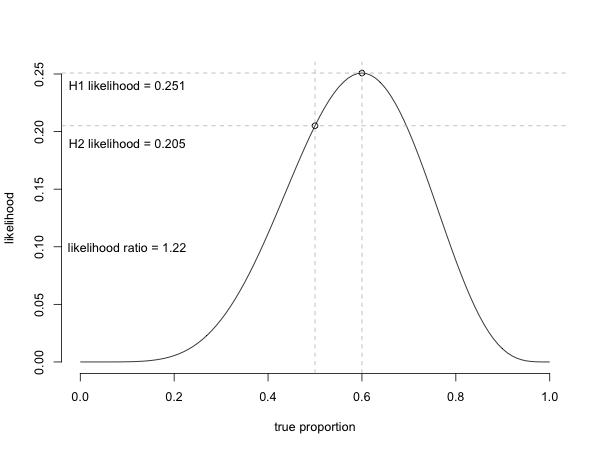
\includegraphics[width=.9\linewidth]{figures/coinFlip.png}
\end{itemize}
\end{itemize}

\item \textbf{Path of belief}: do I really \emph{believe} this coin will come up heads 60\% of the time?
\begin{itemize}
\item No\ldots{}I have \emph{prior} beliefs.
\item One "experiment" with 6 heads does not \emph{change} my prior beliefs
\end{itemize}
\end{enumerate}


These paths form the basis of three dominant statistical paradigms in the psychological literature:
\begin{enumerate}
\item Neyman-Pearson (the most common)
\item Likelihood
\item Bayesian
\end{enumerate}

\begin{enumerate}
\item Neyman-Pearson method
\label{sec-3-1}

Historically, our method of hypothesis testing (using $p$-values) is an amalgamation of two (quite different) ideas from a couple of early 20th century statisticians:

\begin{itemize}
\item Jerzy Neyman: $p$-value tells you what \emph{action} to perform.  If $p<\alpha$, then we reject null hypothesis
\begin{itemize}
\item When we \emph{act} as if there is an effect when $p<0.05$, in the \emph{long run} we won't be wrong more than 5\% of the time
\end{itemize}
\item Ronald Fisher: $p$-value measures evidence\ldots{}the smaller the $p$-value, the greater the evidence (this is actually incorrect)
\item Note: when I teach undergraduate statistics, I teach \emph{only} the Neyman method.  
\begin{itemize}
\item define $H_0$
\item set $\alpha$ (usually 0.05) and find the critical test statistic
\item if test statistic exceeds critical, we we reject $H_0$ (action)
\end{itemize}
\item However, most psychological literature (and many courses) implicitly tack on the incorrect Fisher ideas.  
\begin{itemize}
\item Example: I got $p=0.03$ for "Effect 1" and $p=0.003$ for "Effect 2"..which has "more evidence"?
\item Answer: neither, but Fisher thought Effect 2 would have more evidence
\item this understanding is implicit everywhere in psychology, but it is wrong!
\end{itemize}
\item Goal of Neyman-Pearson method: error control
\begin{itemize}
\item don't make a fool out of yourself in the long run
\end{itemize}
\end{itemize}
\end{enumerate}
% Emacs 25.3.1 (Org mode 8.2.10)
\end{document}